% Отключаем subsection!
\PassOptionsToPackage{subsection=false}{beamerouterthememiniframes}
\documentclass[usenames,dvipsnames,pdftex,unicode,hidelinks]{beamer}
  \usepackage{cmap}
  \usepackage[T2A]{fontenc}
  \usepackage[utf8]{inputenc}
  \usepackage[english,russian]{babel}
  \usepackage{wasysym}
  \usepackage{mathtext} % для кириллицы в формулах
    \DeclareSymbolFont{T2Aletters}{T2A}{cmr}{m}{it} % кириллица в формулах курсивом

  \usepackage{tikz}
    \usetikzlibrary{positioning,fit,backgrounds}
  \graphicspath{{../img/}{../../img/}}

  \usepackage{numprint}
    % алиас и настройки для numprint
    \newcommand{\num}[1]{\numprint{#1}}
    \npthousandsep{\,}
    \npthousandthpartsep{}
    \npdecimalsign{,}

  % add frame number to footline
  \let\oldmacro\insertshorttitle
  \renewcommand*\insertshorttitle{
    \oldmacro\hfill
    -\,\insertframenumber\,- % TODO: temporary comment total count % \,/\,\inserttotalframenumber
  }
  % TODO HACK: вместо института выводим автора
  \renewcommand*\insertshortinstitute{
    \insertshortauthor
  }

  % hide navigation symbols
  \beamertemplatenavigationsymbolsempty

  \usetheme{Szeged}%{Warsaw}
  \usecolortheme{seahorse}
  \usefonttheme{structurebold}
  \useinnertheme{rounded}
  % Патчим некоторые цвета
  %\setbeamertemplate{background canvas}[vertical shading][bottom=black!60!blue,top=black!80!blue]
  \setbeamercolor{block title}{bg=title.bg}
  \setbeamercolor{block body}{bg=title.bg!60}

  \setbeamercovered{transparent}

  \newcommand{\muted}[1]{\textcolor{gray}{#1}}

  \newcommand{\vect}[1]{\vec{#1}} % единое выделение векторов (стрелкой)
  \newcommand{\matx}[1]{\mathbf{#1}} % единое выделение матриц (полужирным)
  \newcommand{\transposed}{\top} % единый знак транспонирования (U+22A4 down tack)
  \newcommand{\conj}[1]{#1^*} % единое обозначение комплексного сопряжения (черта сверху)
  \renewcommand{\le}{\leqslant} % <= с наклонной нижней перекладиной
  \renewcommand{\ge}{\geqslant} % >= с наклонной нижней перекладиной
  \renewcommand{\phi}{\varphi} % phi завитушкой

  \newcommand{\todo}[1]{\textbf{\textcolor{red}{TODO: #1}}}

\title[Система моделирования пластических деформаций биологических объектов]{Информационная система моделирования динамики пластических деформаций биологических объектов}
\author[Иван Новиков]{Новиков Иван Александрович}

\institute{Н1: Информационные технологии}

\date{ 2013 г. }

\begin{document}

  % Local background must be enclosed by curly braces for grouping.
  {
    \usebackgroundtemplate{
      \begin{tikzpicture}[show background rectangle, inner frame sep=-2mm, background rectangle/.style={ draw=none }]
        \node (t) at (0,0) {};% HACK :(
       \node[] at (0,-9) {
         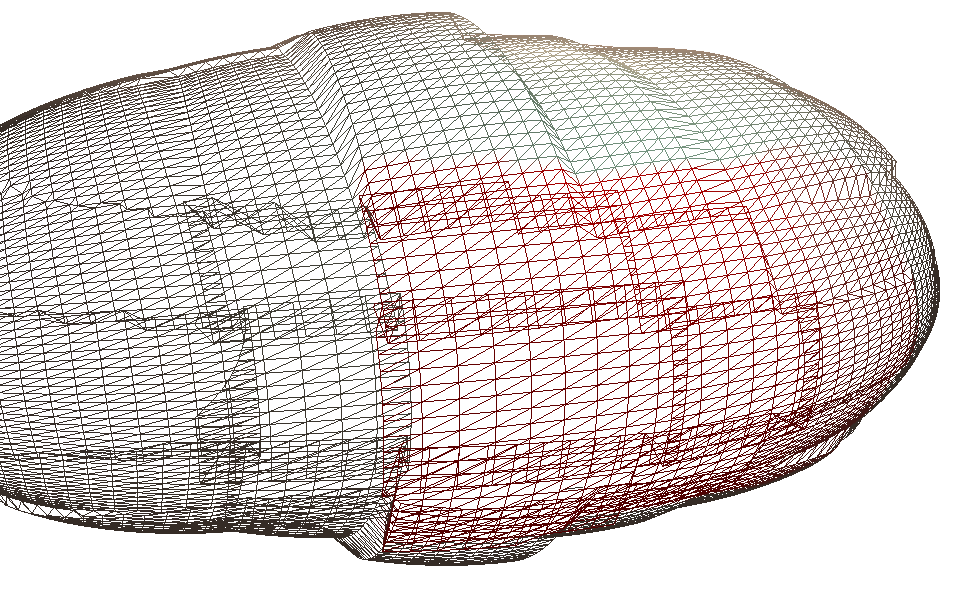
\includegraphics[width=8cm]{screen-big}
       };
      \end{tikzpicture}
    }
    \begin{frame}[plain]
      \titlepage
    \end{frame}
  }

  \section{Постановка задачи}
  \subsection{Постановка задачи} % NB: subsection отключены! Эти имена не будут отображаться
  \begin{frame}{Применения моделирования деформаций}
    % Уменьшаем margin сверху (см. http://tex.stackexchange.com/a/73522/24732)
    \vspace{-2\baselineskip}
    \begin{columns}[c]
      \begin{column}{0.5\textwidth}<-1>
        \begin{center}
          Компьютерные игры
          \only<1>{ 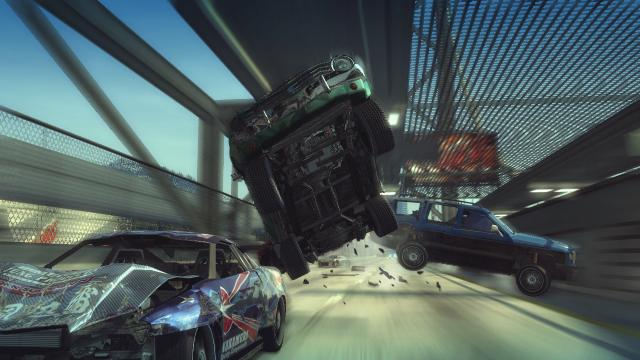
\includegraphics[height=0.3\textheight]{game} }
          % TODO честная полупрозрачность
          \only<2>{ 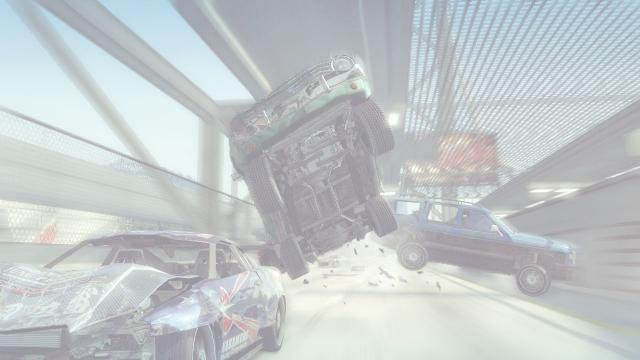
\includegraphics[height=0.3\textheight]{game-phantom} }

          Спецэффекты в кино

          \only<1>{ 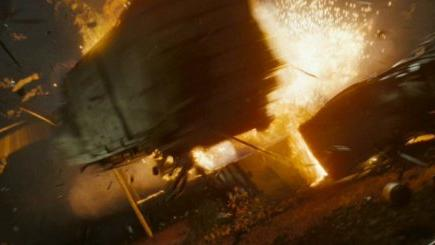
\includegraphics[height=0.3\textheight]{movie} }
          % TODO честная полупрозрачность
          \only<2>{ 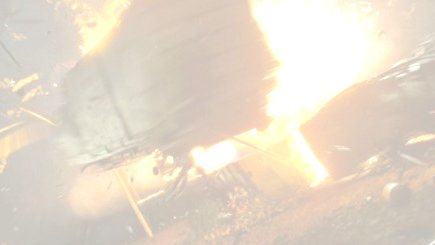
\includegraphics[height=0.3\textheight]{movie-phantom} }
        \end{center}
      \end{column}
      \begin{column}{0.5\textwidth}<-2>
        \begin{center}
          Обучающие тренажёры

          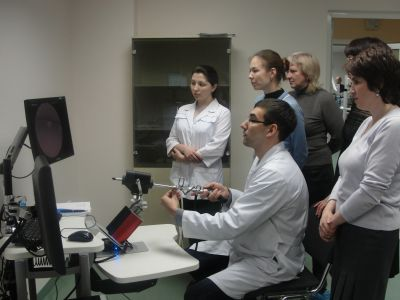
\includegraphics[height=0.3\textheight]{trainer}

          Системы авт. проектирования

          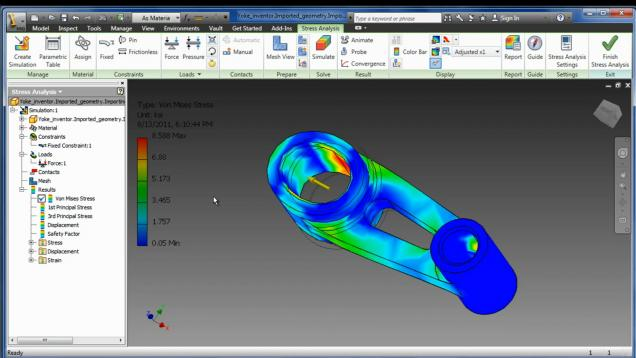
\includegraphics[height=0.3\textheight]{cad}
        \end{center}
      \end{column}
    \end{columns}
  \end{frame}
  \begin{frame}{Моделирование в реальном времени}
    В приложениях, связанных с визуализацией:
    \begin{enumerate}
      \item \alert{Мягкое} реальное время.
      \item Комфорт пользователя: FPS $\ge 30$.
      \item За $\Delta t \le 33$~мс --- \emph{все} расчёты очередного кадра.
      \item На моделирование деформаций отводится \alert{$\Delta t' \approx 3..10$~мс}.
    \end{enumerate}

    \vspace{5mm}

    \begin{center}
      \begin{tikzpicture}[scale=1]
        \fill[Gray!50] (0,0) circle (1);
        \node at (0,0) {1 сек};

        \fill[Gray!50] (3, 0) circle (1);
        \fill[OliveGreen] (3, 0) -- +(0, 1) arc (90:78:1) -- cycle;
        \foreach \a in {6,18,...,359}
          \draw[thin, Gray!75] (3, 0) -- +(\a:1);
        \node[below,OliveGreen] at (3,0) {$\frac1{30}$ с};

        \fill[OliveGreen] (6, 0) circle (1);
        \fill[Red!50] (6, 0) -- +(0, 1) arc (90:54:1) -- cycle;
        \node[below,Red!50] at (6,0) {3 мс};
      \end{tikzpicture}
    \end{center}
  \end{frame}

  \begin{frame}{Актуальность}
    Разработка такой системы актуальна:
    \begin{itemize}
      \item применение систем виртуальной реальности в~обучении;
        % NB: сказать про перспективы 3D-печати тканей,органов...
      \item потребность в САПР протезов, имплантатов;
      \item отсутствие отечественных аналогов.
    \end{itemize}

    \vspace{0.5cm}

    \uncover<2->{
    Недостатки зарубежных аналогов (ANSYS, DEFORM-3D):
    \begin{itemize}
      \item не адаптированы для биологических объектов;
      \item нельзя применить к расчётам в реальном времени;
      \item высокая цена.
    \end{itemize}
    }
  \end{frame}

  \begin{frame}{Цель}
    \begin{block}{Цель проекта}
      Разработка \alert{системы моделирования} пластических деформаций биологических объектов
      \alert{в~реальном времени}.
      % (которая может быть использована как отдельно, так и в качестве
      % \alert{модуля} для встраивания в стороннее приложение)
    \end{block}

    \vspace{0.5cm}

    Задачи:
    \begin{enumerate}
      \item Разработка \textcolor{ForestGreen}{алгоритма} моделирования
      \item \textcolor{ForestGreen}{Его} реализация в виде \textcolor{RoyalPurple}{программной библиотеки}
      \item Разработка на \textcolor{RoyalPurple}{её} основе \textcolor{NavyBlue}{интерактивного приложения}
    \end{enumerate}
  \end{frame}

  \section{Содержание проекта}
  \subsection{Содержание проекта}
  \begin{frame}{Научная новизна}
    \begin{enumerate}
      \setlength{\itemsep}{5mm}
      \item Собственные наработки по моделированию деформаций:

        \hspace{7mm}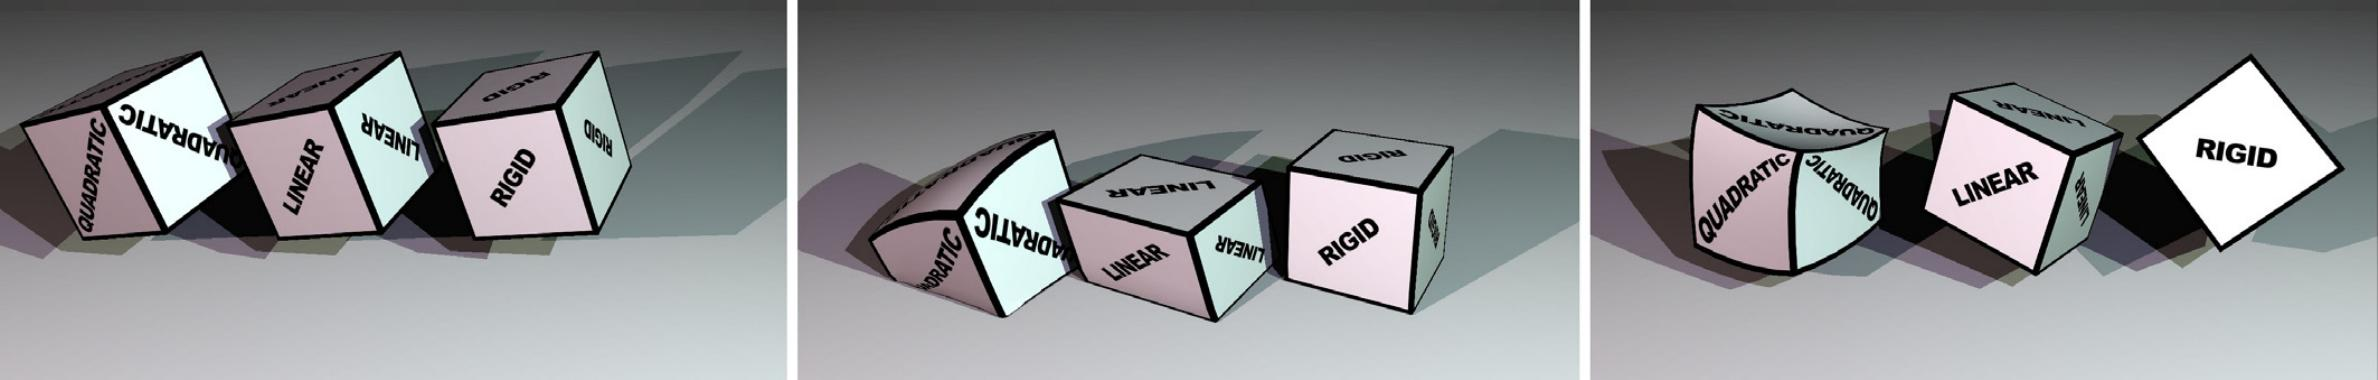
\includegraphics[height=15mm]{meshless}
        \begin{itemize}
          \item объединение физических методов с геометрическими;
          % \item разбиение 3D-модели на кластеры, подбор оптимального линейного преобразования для каждого;
          \item минимум ограничений на 3D-модель объекта
          \item применение графического процессора.
        \end{itemize}
      \item Гибкий программный интерфейс (API).
      \item Адаптация алгоритма к физическим свойствам биологических объектов.
    \end{enumerate}
  \end{frame}

  \begin{frame}{Созданный задел}
    Публикации:
    {
      \scriptsize
      \begin{enumerate}
        \item
          \textbf{И.А.~Новиков}, Д.А.~Гладкий. Система моделирования деформаций неупругих тел в реальном времени~//
          Материалы XLIX МНСК <<Студент и научно-технический прогресс>>, Физика. --- Новосибирск:
          НГУ, 2011.
        \item
          \textbf{I.A~Novikov}, M.Y~Fursov, I.E.~Efremov. UGENE Assembly Browser: a tool for NGS data
          visualization~// Abstracts of VIII BGRS. "--- Novosibirsk, 2012.
        \item
          Л.Р.~Григорьян, \textbf{И.А.~Новиков}. Информационная система обработки прецизионных сигналов~//
          Коллективная монография. Современные проблемы физики, биофизики и инфокоммуникационных технологий.
          --- Краснодар: ЦНТИ, 2013. С. 185 - 198.
        %\item
        %  \textbf{И.А.~Новиков}, Л.Р.~Григорьян. Информационная система
        %  обработки прецизионных сигналов~// Современное состояние и приоритеты развития
        %  фундаментальных наук в регионах. Труды X Всероссийской научной конференции
        %  молодых ученых и студентов. "--- Краснодар, 2013
      \end{enumerate}
    }
    Интеллектуальная собственность:
    {
      \scriptsize
      \begin{enumerate}
        \item
          Программа ProcessData. Свидетельство о государственной регистрации программы
          для ЭВМ №2013612036 от 12.02.2013~г.
        \item
          Программа графической визуализации и анализа данных медицинских измерений.
          Свидетельство о государственной регистрации программы для ЭВМ №2013618780 от 18.09.2013~г.
      \end{enumerate}
    }
    Создан работающий прототип системы.
  \end{frame}

  \begin{frame}{Работающий прототип}
    \begin{center}
      \only<1>{ 1. До удара \\ 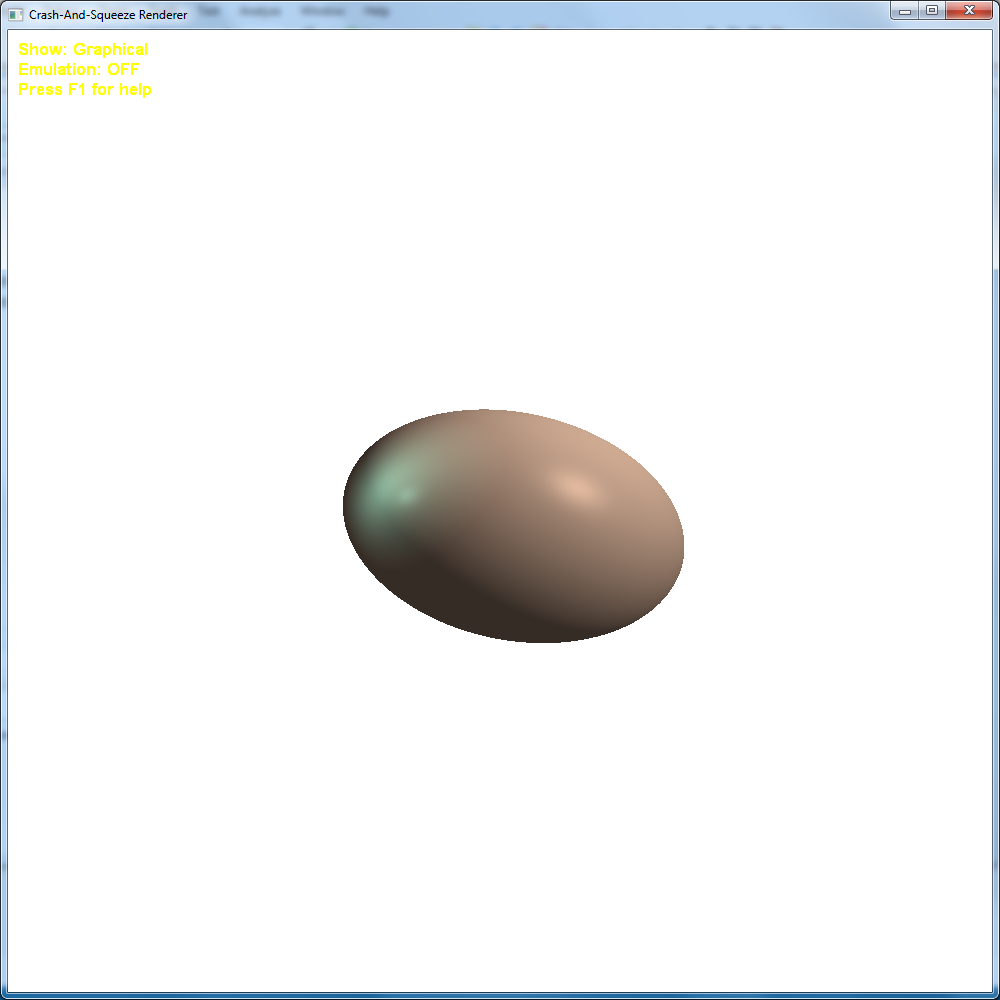
\includegraphics[height=0.7\textheight]{screen-0} }
      % TODO более сильная деформация
      \only<2>{ 2. Вскоре после удара \\ 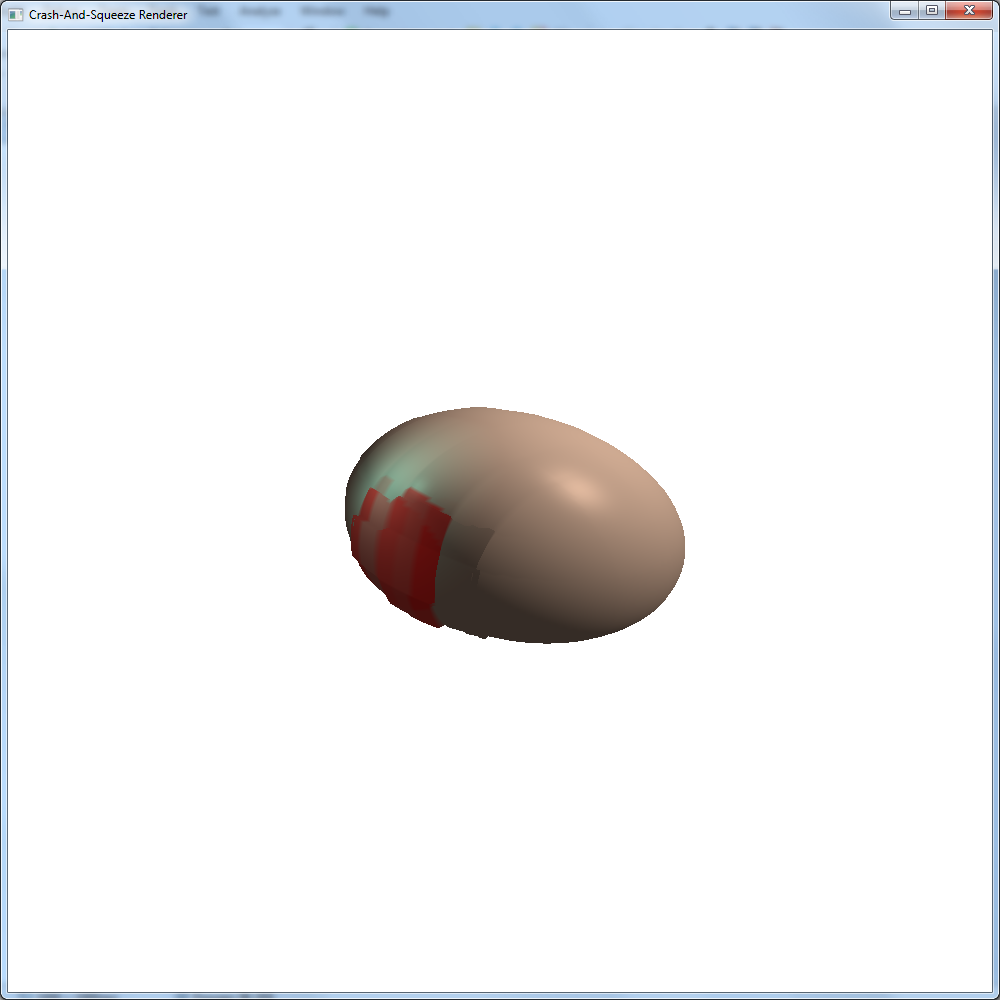
\includegraphics[height=0.7\textheight]{screen-1} }
      \only<3>{ 3. После удара \\ 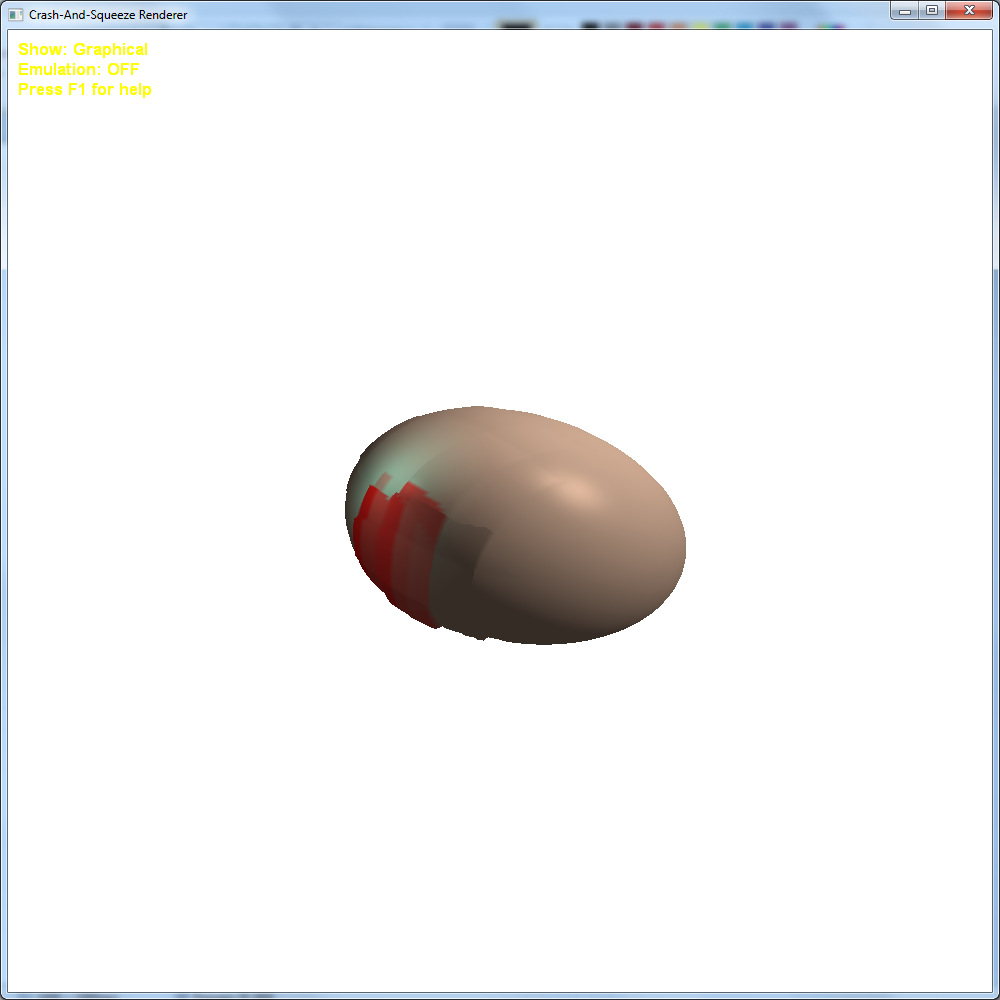
\includegraphics[height=0.7\textheight]{screen-2} }
    \end{center}
  \end{frame}

  \begin{frame}{Потенциальные заказчики}
    \begin{itemize}
      \setlength{\itemsep}{5mm}
      \item Учебные заведения

        \foreach \name in {ksma, kubsu, kubstu} {
          \hspace{5mm}\includegraphics[height=15mm]{\name}
        }
      \item Научные организации

        \foreach \name in {ramn} {
          \hspace{5mm}\includegraphics[height=10mm]{\name}
        }
      \item Разработчики САПР

        \foreach \name in {nanocad, ascon, rusapr} {
          \hspace{5mm}\includegraphics[height=10mm]{\name}
        }
    \end{itemize}
  \end{frame}

  \begin{frame}{Коммерциализация}
    Две формы продукта:

    \begin{enumerate}
      \setlength{\itemsep}{5mm}
      \item Модуль для встраивания в стороннее приложение
        \begin{itemize}
          \item Основные потребители: разработчики САПР
          \item Примерный объем рынка: 50--100 лицензий
          \item Стоимость лицензии: $\approx 300$ тыс. руб.
        \end{itemize}
      \item Автономное приложение \textcolor{Gray}{(основанное на этой библиотеке)}
        \begin{itemize}
          \item Основные потребители: высшие учебные заведения
          \item Примерный объем рынка: 1000--2000 лицензий
          \item Стоимость лицензии: $\approx 15$ тыс. руб.
        \end{itemize}
    \end{enumerate}
  \end{frame}

  \section{План проекта}
  \subsection{План проекта}
  \begin{frame}{Календарный план}
    1\textsuperscript{й} год:
    \begin{enumerate}
      \item Разработка алгоритма моделирования деформаций.
      \item Создание библиотеки, реализующей алгоритм.
      \item Тестирование, в т.\,ч. на 3D-моделях реальных объектов.
      \item Разработка графического интерфейса приложения.
    \end{enumerate}
    \uncover<2->{
      Дальнейшее развитие:
      \begin{itemize}
        \item Оптимизация, более глубокое использование GPU
        \item Разработка дополнительных инструментов
          \par{
            \scriptsize
            (конвертация из различных форматов 3D-моделей,\\
            задание физических свойств прямо в 3D-редакторе и т.\,п.)
          }
        \item Поддержка возможности расширения системы
          \par{
            \scriptsize
            (добавление новых алгоритмов, обработчиков событий и т.\,п.)
          }
      \end{itemize}
    }
  \end{frame}

  \begin{frame}{Перспективы и риски}
    Перспективы:
    \begin{itemize}
      \item Поддержка аппаратной части обучающих тренажёров
        \par{
          \scriptsize
          --- сотрудничество с НИИ
        }
      \item Интеграция в популярные САПР
        \par{
          \scriptsize
          --- сотрудничество с разработчиками
        }
    \end{itemize}

    Риски:
    \begin{itemize}
      \item Аппаратная несовместимость
        \par{
          \scriptsize
          $\Longrightarrow$ добавление режима совместимости
        }
      \item Консервативность потребителей
        \par{
          \scriptsize
          $\Longrightarrow$ демонстрация, реклама, опытное апробирование
        }
      \item Интеллектуальная собственность
        \par{
          \scriptsize
          $\Longrightarrow$ регистрация авторских свидетельств на ПО и алгоритм
        }
    \end{itemize}
  \end{frame}

  \begin{frame}{Конечный результат}
    \begin{itemize}
      \setlength{\itemsep}{5mm}
      \item Алгоритм моделирования пластических деформаций биологических объектов в
        реальном времени
      \item Программный модуль (библиотека), реализующий алгоритм, с гибким интерфейсом (API)
      \item Графическое приложение для запуска моделирования \\(на основе этой библиотеки)
      \item \emph{(В перспективе)} Вспомогательные инструменты
    \end{itemize}
  \end{frame}


  % Заканчиваем последний section, чтобы заключение, "спасибо" и запасные слайды к нему не
  % относились и не отображались в навигации сверху
  \section{}

  \begin{frame}[plain]
    \begin{center}
      { \Huge Спасибо за внимание! }

      \vspace{1cm}

      Иван Новиков\\
      \url{http://about.me/moonlighter}\\
      \href{mailto:nia.afti@gmail.com}{\nolinkurl{nia.afti@gmail.com} }

    \end{center}
  \end{frame}

  % Запасные слайды

  \begin{frame}{Производительность}
    \begin{center}
      {
        \tiny
        Intel Core 2 Quad Q6660 2.4 GHz, NVIDIA GeForce 8800 GTX
      }

      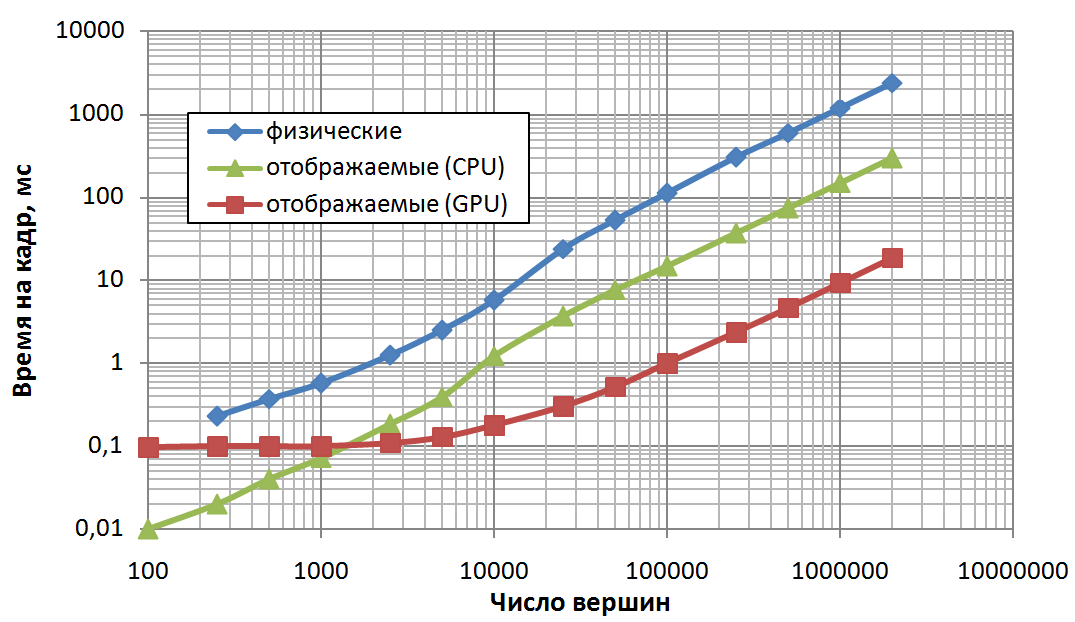
\includegraphics[height=0.7\textheight]{time-plot}

      {
        \scriptsize
        За \alert{3 мс}/кадр: до \alert{\num{6000}} физ. точек и до \alert{\num{200000}} отображаемых вершин
      }
    \end{center}
  \end{frame}

  \begin{frame}{Использование в обучении}
    \begin{tikzpicture}[scale=1.5]
      \tikzstyle{block} = [rectangle, draw=blue, rounded corners, fill=cyan!10,
                           text centered, text width=2.3cm, font=\footnotesize, minimum height=4em]
      \tikzstyle{bblck} = [block, minimum height=3em, draw=Green, fill=LimeGreen!30]
      \tikzstyle{tblck} = [block, minimum height=3em, draw=Plum, fill=BlueViolet!10]
      \tikzstyle{mblck} = [block, minimum height=3em, draw=RedOrange, fill=Red!10]
      \tikzstyle{last} = [text width=3cm, font=\scriptsize]

      \node[block] (root) {Высшее образование};
      \node[tblck] (tech) [right=1.0cm of root] {Биотехнологии};
      \node[bblck] (bio)  [above=0.3cm of tech] {Биология};
      \node[mblck] (med)  [below=0.3cm of tech] {Медицина};

      \node[bblck,last] (bio1) [right=1.0cm of bio]  {Моделирование тканей};
      \node[bblck,last] (bio2) [above=0.2cm of bio1] {Механика движения};

      \node[tblck,last] (tech1)[right=1.0cm of tech] {Имплантация, протезирование};

      \node[mblck,last] (med1) [right=1.0cm of med]  {Моделирование органов в движении};
      \node[mblck,last] (med2) [below=0.2cm of med1] {Моделирование воздействий на ткани};

      \foreach \nd/\n in {bio/2,tech/1,med/2} {
        \draw[->, thick] (root) -- (\nd);
        \foreach \x in {1,...,\n}
          \draw[->, thick] (\nd) -- (\nd\x);
      }
    \end{tikzpicture}
  \end{frame}

  \begin{frame}{Другие области применения}
    \begin{itemize}
      \setlength{\itemsep}{5mm}
      \item Компьютерное моделирование крэш-тестов
        \begin{itemize}
          \item Существующие системы моделируют только деформацию автомобиля
        \end{itemize}

      \item Компьютерные игры
        \begin{itemize}
          \item Отечественные производители игр пока сильно отстают от зарубежных
        \end{itemize}

      \item Другие системы виртуальной реальности
        \begin{itemize}
          \item Кроме тренажёров также развиваются виртуальные музеи, интерактивные образовательные
            программы, ...
        \end{itemize}
    \end{itemize}
  \end{frame}

\end{document}

